% documentclass options:
\documentclass[11pt,
  a4paper,
  parskip=half, % This is some extra vertical space between paragraphs, the suggestion is 2cm which is really ugly, so we use what koma script gives us
  % you can also set it to full for even more space. But there is a bad tex style decision: parskip also changes the spacing between listitems such as
  % enumerate and itemize. For this purpose we include the enumitem package and set itemsep=.5em, of course you can change this
  BCOR=10mm, % BCOR is binding correction
  english,
  % if you'd rather have a one sided thesis, add `oneside' to the documentclass
  % oneside,
  % ngerman is needed for hyphenation if the thesis contains parts written in German, switch order with english if you write mainly in English.
  % Remember to change order in the babel package (below) as well.
  % Last language is the preferred one.
  english]{scrbook}
\usepackage[english]{babel} % If you write mainly in English change order to ngerman, english. Also change that in the documentclass options above.
% Include of titling must happen before \title etc.
% that's why it's not in setup.tex
\usepackage{titling}
\title{Ultrasonic Ray Tracing Simulation for Indoor Localization and Mapping Applications}
\author{Marko Gucanin}

% Change to your first examiner
% The ~ enables non sentence spacing after a period
\newcommand{\firstexaminer}{Prof.~Dr.~Christian Schindelhauer}
% Change to your second examiner, some undergraduate studies don't have a second examiner
% in this case just comment out the following line
\newcommand{\secondexaminer}{Prof.~Dr.~Leonhard Reindl}
% Change to your advisers
% \newcommand{\advisers}{Prof.~Dr.~Christian Schindelhauer}

% include all packages and define commands in setup.tex

%------------------------------------------------------------------------------
%       package includes
%------------------------------------------------------------------------------
    % font encoding is set up for pdflatex, for other environments see
    % http://tex.stackexchange.com/questions/44694/fontenc-vs-inputenc
    \usepackage[T1]{fontenc}  % 8-bit fonts, improves handling of hyphenations
    \usepackage[utf8x]{inputenc}
    % provides `old' commands for table of contents. Eases the ability to switch
    % between book and scrbook
    \usepackage{scrhack}


    % ------------------- layout, default -------------------
    % adjust the style of float's captions, separated from text to improve readabilty
    \usepackage[labelfont=bf, labelsep=colon, format=hang, textfont=singlespacing]{caption}
    % With format = hang your caption will look like this:
    % Figure 1: Lorem ipsum dolor sit amet,
    %           consectetuer adipiscing elit.
    %           Ut purus elit, vestibulum
    % If you instead want
    % Figure 1: Lorem ipsum dolor sit amet,
    % consectetuer adipiscing elit. Ut purus
    % elit, vestibulum
    % change to format=plain
    \usepackage{chngcntr}  % continuous numbering of figures/tables over chapters
    \counterwithout{equation}{chapter}
    \counterwithout{figure}{chapter}
    \counterwithout{table}{chapter}

    % Uncomment the following line if you switch from scrbook to book
    % and comment the setkomafont line
    %\usepackage{titlesec}  % remove "Chapter" from the chapter title
    %\titleformat{\chapter}[hang]{\bfseries\huge}{\thechapter}{2pc}{\huge}
    \setkomafont{chapter}{\normalfont\bfseries\huge}

    \usepackage{setspace}  % Line spacing
    \onehalfspacing
    % \doublespacing  % uncomment for double spacing, e.g. for annotations in correction

    % ------------------- functional, default-------------------
    \usepackage[dvipsnames]{xcolor}  % more colors
    \usepackage{array}  % custom format per column in table - needed on the title page
    \usepackage{graphicx}  % include graphics
    \usepackage{subfig}  % divide figure, e.g. 1(a), 1(b)...
    \usepackage{amsmath}  % |
    \usepackage{amsthm}   % | math, bmatrix etc
    \usepackage{amsfonts} % |
    \usepackage{calc}  % calculate within LaTeX
    \usepackage[unicode=true,bookmarks=true,bookmarksnumbered=true,
                bookmarksopen=true,bookmarksopenlevel=1,breaklinks=false,
                pdfborder={0 0 0},backref=false,colorlinks=false]{hyperref}
    \usepackage{etoolbox} % if-else commands


    %==========================================
    % You might not need the following packages, I only included them as they
    % are needed for the example floats
    % ------------------- functional, custom -------------------
    \usepackage{algorithm,algpseudocode}
    \usepackage{bm}  % bold greek variables (boldmath)
    \usepackage{tikz}
    \usetikzlibrary{positioning}  % use: above left of, etc
    
    % Required for the ToDo list.
    \usepackage{ifthen}

    % Improves general appearance of the text
    \usepackage[protrusion=true,expansion=true, kerning]{microtype}
    \usepackage{enumitem}
    % Nicer font for pdf rendering.
    %\usepackage{lmodern}
    
    % For nicer looking tables.
    \usepackage{booktabs}

    % You don't need this, just for demonstration of a longer caption.
    \usepackage{lipsum}

%------------------------------------------------------------------------------
%       (re)new commands / settings
%------------------------------------------------------------------------------
    % ----------------- referencing ----------------
    \newcommand{\secref}[1]{section~\ref{#1}}
    \newcommand{\chapref}[1]{chapter~\ref{#1}}
    \renewcommand{\eqref}[1]{equation~(\ref{#1})}
    \newcommand{\figref}[1]{figure~\ref{#1}}
    \newcommand{\tabref}[1]{table~\ref{#1}}

    % ------------------- colors -------------------
    \definecolor{darkgreen}{rgb}{0.0, 0.5, 0.0}
    % Colors of the Albert Ludwigs University as in
    % https://www.zuv.uni-freiburg.de/service/cd/cd-manual/farbwelt
    \definecolor{UniBlue}{RGB}{0, 74, 153}
    \definecolor{UniRed}{RGB}{193, 0, 42}
    \definecolor{UniGrey}{RGB}{154, 155, 156}


    % ------------------- layout -------------------
    % prevents floating objects from being placed ahead of their section
    \let\mySection\section\renewcommand{\section}{\suppressfloats[t]\mySection}
    \let\mySubSection\subsection\renewcommand{\subsection}{\suppressfloats[t]\mySubSection}



    % ------------------- math formatting commands -------------------
    % define vectors to be bold instead of using an arrow
    \renewcommand{\vec}[1]{\mathbf{#1}}
    \newcommand{\mat}[1]{\mathbf{#1}}
    % tag equation with name
    \newcommand{\eqname}[1]{\tag*{#1}}


    % ------------------- pdf settings -------------------
    % ADAPT THIS
    \hypersetup{pdftitle={\thetitle},
                pdfauthor={\theauthor},
                pdfsubject={},
                pdfkeywords={},
                pdfpagelayout=OneColumn, pdfnewwindow=true, pdfstartview=XYZ, plainpages=false}


    %==========================================
    % You might not need the following commands, I only included them as they
    % are needed for the example floats

    % ------------------- Tikz styles -------------------
    \tikzset{>=latex}  % arrow style


    % ------------------- algorithm ---------------------
    % Command to align comments in algorithm
    \newcommand{\alignedComment}[1]{\Comment{\parbox[t]{.35\linewidth}{#1}}}
    % define a foreach command in algorithms
    \algnewcommand\algorithmicforeach{\textbf{foreach}}
    \algdef{S}[FOR]{ForEach}[1]{\algorithmicforeach\ #1\ \algorithmicdo}

    % line spacing should be 1.5
    \renewcommand{\baselinestretch}{1.5}

    % set distance between items in a list, for more details see the
    % enumitem package: https://www.ctan.org/pkg/enumitem
    \setlist{itemsep=.5em}
    
    % use ra in your tables to increase the space between rows
    % 1.3 should be fine
    \newcommand{\ra}[1]{\renewcommand{\arraystretch}{#1}}

	% ToDo counters
	\usepackage{ifthen} %für whiledo-Schleife
	\newcounter{todos}
	\setcounter{todos}{0}
	\newcounter{extends}
	\setcounter{extends}{0}
	\newcounter{drafts}
	\setcounter{drafts}{0}

	% ------------------- marker commands -------------------
    % ToDo command
    \newcommand{\todo}[1]{\textbf{\textcolor{red}{(TODO: #1)}}\refstepcounter{todos}\label{todo \thetodos}}
	\newcommand{\extend}[1]{\textbf{\textcolor{darkgreen}{(EXTEND: #1)}}\refstepcounter{extends}\label{extend \theextends}}
	% Lighter color to note down quick drafts
	\newcommand{\draft}[1]{\textbf{\textcolor{NavyBlue}{(DRAFT: #1)}}\refstepcounter{drafts}\label{draft \thedrafts}}
	
	% microtype with lmodern, see https://tex.stackexchange.com/questions/75305/microtype-warning-with-lmodern-package-and-koma-script
    %\DeclareMicrotypeAlias{lmss}{cmr}
    
    % Variable definitions
    \newenvironment{conditions}
    {\par\vspace{\abovedisplayskip}\noindent\begin{tabular}{>{$}l<{$} @{${}={}$} l}}
    {\end{tabular}\par\vspace{\belowdisplayskip}}

\begin{document}
    \pagestyle{empty} % no header and no page number
    % disable hyper links to remove warning "destination with same identifier"
    % this means within this section nothing can be referenced with a hyperlink
    \hypersetup{pageanchor=false}

    % enable/disable, depending on your chosen language
    \begin{titlepage}
\begin{center}

\newcommand{\HorizontalLine}{\rule{\linewidth}{0.3mm}}

{\Large Master's Thesis}\\[1.3cm]


% _____________________________________________________________________________
\HorizontalLine \\[0.4cm]
% Write your title in a fancy way like this if you want to customize it, otherwise simply let tex do it for you
% \begin{spacing}{3}
%     {\huge \bfseries The Long, Long } \\
%     {\huge \bfseries Long Long} \\
%     {\huge \bfseries Title}\\
% \end{spacing}
{ \huge \bfseries \thetitle }
\HorizontalLine \\[1.5cm]
% _____________________________________________________________________________


{\Huge \theauthor} \\[2cm]


\begin{tabular}[hc]{>{\huge}l >{\huge}l}
  Examiners: & \firstexaminer \\[0.3cm]
             & \secondexaminer\\[0.3cm]
%   Advisers: & \advisers \\[1.2cm]
\end{tabular}
\vfill  % move the following text to the bottom

\Large {
    Albert-Ludwigs-University Freiburg\\
    Faculty of Engineering\\
    Department of Computer Science\\
    Chair of Computer Networks and Telematics\\[1cm]

    November 6\textsuperscript{th}, 2020\\
}
\end{center}
\end{titlepage}

\thispagestyle{empty}
% title page back
\ \vfill \ \\  % at least one space required before vfill
\
\textbf{Writing Period}            \smallskip{} \\
06.\,05.\,2020 -- 06.\,11.\,2020   \bigskip{} \\
\
\textbf{Examiner}                  \smallskip{} \\
\firstexaminer                     \bigskip{} \\
\
% If there is a second examiner include it
\ifdef{\secondexaminer}
	{
	% Include
	\textbf{Second Examiner}       \smallskip{} \\
	\secondexaminer                \bigskip{} \\
	\
	}
	{
	% No second examiner, ignore
	}
% \textbf{Advisers}                  \smallskip{} \\
% \advisers

    \pagestyle{plain} % remove chapter name from top, page number at the bottom
    % use \pagestyle{headings} for having the chapter on top of the pages
    % if you wang a more fancy header use \usepackage[automark,headsepline]{scrlayer-scrpage}
    % and read about it in the KOMA script documentation, https://www.ctan.org/pkg/koma-script
    \frontmatter  % roman page numbers
    % Copied from the official declaration from the examination office (typos fixed).
% Please double check the wording on their website and report changes.
% (https://www.tf.uni-freiburg.de/de/studium-lehre/a-bis-z-studium/dokumente/Declarationforthefinalthesis.pdf)

\chapter*{Declaration}

I hereby declare, that I am the sole author and composer of my thesis and that no other sources or learning aids, other than those listed, have been used. 
Furthermore, I declare that I have acknowledged the work of others by providing detailed references of said work.  \newline
I also hereby declare that my thesis has not been prepared for another examination or assignment, either in its entirety or excerpts thereof.
\\[3\normalbaselineskip]
\begin{tabular}{p{\textwidth/2} l}
  \rule{\textwidth/3}{0.4pt}   &   \rule{\textwidth/3}{0.4pt} \\
  Place, Date                  &   Signature
\end{tabular}

    \chapter*{Abstract}
This thesis deals with the problem of generating test data for indoor localization and mapping systems using acoustic sources (speakers) and receivers (microphones) in a given environment.
In particular methods of ray tracing and ultrasonic path evaluation will be explored and presented.
The suggested methods have been implemented in an Acoustic Ray Tracing Simulator (ARTS).
\newline ARTS is able to generate test sample data for a set of receivers by approximating the propagation of sound waves from acoustic sources as rays in a 3D modeled environment.
The geometry of the environment is provided by 3D data from tools which support the Wavefront OBJ file format.
Using this data and the geometric ray tracing method, reflections up to third order are being computed and sampled at the receivers end.
The sampled data can then be used in localization or mapping systems to evaluate different environments and setups.

    \tableofcontents
    \listoffigures
    \listoftables
    % \listofalgorithms
    \hypersetup{pageanchor=true}  % re-enable hyperlinking

    \mainmatter  % Arabic page numbers
    \chapter{Introduction}\label{chap:introduction}
Indoor environments pose various challenges for localization and mapping algorithms, mainly because many unique settings exist.
Finding a solution which works for a lot of setups is therefore rather difficult. \newline
Let's start by giving an example for a typical indoor localization and mapping problem and then move on to describe the common problem on a higher level.\newline
Sometimes, finding your smartphone at home might be harder than you think, especially if you have no clue where you left it.
If nothing helps you will probably ask a family member, room mate or partner to help you out with a phone call.
Once you hear the sound of your exotic ring tone you will most likely start following it until you find your phone. \newline
This might sound like a silly example but in fact it covers the basic elements of a localization problem: A set of receivers (ears), an environment (house or apartment) and the unknown location of a source (smartphone).\newline
J. Bordoy et al. proposed a solution for almost the same problem \cite{bordoy2019exploiting}. 
They used a combination of direct path and reflected ultrasound signals. 
Former is usually referred to as line-of-sight (LOS) and latter as non-light-of-sight (NLOS) scenario.
LOS describes the case where a localization system is able to "see" the source to be located and NLOS is the case where an object/obstacle is blocking the direct path between the localization system and the source.\newline
Let's move on to an indoor mapping/imaging example from Flávio Ribeiro et al. where they try to estimate the geometry of a room with compact microphone arrays \cite{ribeiro2011geometrically}. 
The source, in this case a loudspeaker, is co-located with the receiver array. 
A known test signal is emitted through the source and the reflections of the test signal are used to estimate the room geometry. 
Since they apply directional constraints on the received signal, they are able to extract the relevant reflections and therefore estimate the dimensions of the room.\newline
Even though both of these proposals are trying to solve two completely different problems, they share a common "interface" to the physical world. 
This interface is illustrated in \figref{fig:Intro}.

\begin{figure}[H]
    \begin{center}
    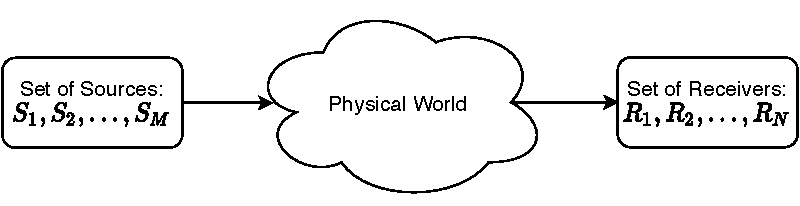
\includegraphics[width=\textwidth]{figures/introduction/figIntro.pdf}
    \end{center}
    \caption[Problem Generalization]{Problem Generalization}
    \label{fig:Intro}
\end{figure}

The sources emit a signal through the room and interact with the environment. 
Effects like path attenuation, reflections, scattering and diffraction will modify the signal as it propagates through the room \cite{vorlander2013computer}.
The result of these effects is perceived and recorded by the receivers.
Modelling and simulating the sources, receivers, the environment, the effects and the receivers will enable creating test data for the problems like \cite{bordoy2019exploiting} and \cite{ribeiro2011geometrically}.
Tests can be performed and evaluated in virtual environments and setups.
Creating a tool which allows us to do these things is therefore very useful.
The question is, how can this be achieved?

One very promising answer to this question is Acoustic/Ultrasonic Ray Tracing.
The hearing range of humans is $20\text{Hz} < f < 20 \text{kHz}$ and will be called "audible spectrum".
For frequencies higher than $20\text{kHz}$ we enter the ultrasound spectrum.
A lot of the general acoustic laws for the audible spectrum apply for the ultrasound spectrum as well.
There are however two main differences which are very important when designing an indoor localization or mapping system:\newline
1. Imagine having a system which depends on audible sound waves.
If the system is to be used in a human inhabited indoor environment, the system could be very annoying to people, especially for periodic sources.
This statement however is purely subjective and based on reasonable common sense.
Nonetheless it is a practical reason not to use frequencies below 20kHz.\newline
2. The second reason is that ultrasound waves can be approximated by rays, because of their reflection behavior.
This is mainly due to the fact that the relation between wavelength and the size of a reflecting surface is important.
For 20kHz the wavelength is approximately 17mm and for 100kHz it's approximately 3.4mm.
If the surface is much larger than the wavelength, which is the case for a lot of objects and obstacles, it will most likely get reflected.

This thesis explores this geometrical approach in order to provide simulated reflection data for indoor systems like \cite{bordoy2019exploiting} and \cite{ribeiro2011geometrically}.

    \chapter{Related Work}\label{chap:relatedwork}

\textbf{Articles}\newline
\cite{rober2007ray} \textit{Niklas Röber et al. "Ray acoustics using computer graphics technology"} \newline
Most of the ideas for this thesis are based on the geometric acoustic approach of this paper.
For higher frequencies the geometric acoustic approach seems very promising and can be efficiently realized with GPU acceleration.
The room impulse response (RIR) method is especially beneficial for generating test data for TDOA or AOA systems.

\cite{rindel1995computer} \textit{Jens Holger Rindel, "Computer simulation techniques for acoustical design of rooms"} \newline
This paper has been found on the website of ODEON and displays a ray tracing, an image source and a hybrid method for room acoustic simulations.
The presented Image Source Method has been the main driver and approach for ARTS.

\textbf{Implementations}\newline
\cite{odeon} \textit{Odeon A/S, ODEON} \newline
ODEON is a commercial software for simulating and measuring indoor room acoustics of buildings.
Some of the above mentioned articles and their methods have been used to build ODEON.
It features a rich database of materials with absorption coefficients.

\cite{wayverb} \textit{Reuben Thomas, Wayverb} \newline
Wayverb is an open source software for room acoustics, similar to ODEON.
Some of the ideas have been used in this thesis as well, especially the geometric image-source method.
It is currently only supported on OSX and needs porting for other platforms.
Unfortunately it has been discovered pretty late in the project process.
It would have been a very good starting point as it seems to be very promising and worth looking into for indoor localization and mapping problems.

    \chapter{Background}\label{chap:background}
In this chapter we will briefly introduce some basic model definitions and notation conventions for the following chapters.

\section{Basic Model Definitions and Notations}\label{sec:backgroundBasic}
A Setup $A$ is defined by
\begin{itemize}
    \item a set $S$ of $M$ Sources: $S=\{S_1,S_2,...,S_M\}$,
    \item a set $R$ of $N$ Receivers: $R=\{R_1,R_2,...,S_N\}$,
    \item a set $Q$ of $K$ Obstacles: $Q=\{Q_1,Q_2,...,Q_K\}$ and
    \item a tuple of physical properties: $(\vartheta,\phi, p)$
\end{itemize}
where
\begin{conditions}
    M           & number of source nodes, $M \in \mathbb{N}$ \\
    N           & number of receiver nodes, $N \in \mathbb{N}$ \\
    K           & number of obstacles, $K \in \mathbb{N}$ \\
    \vartheta   & temperature in $[^{\circ}\textrm{C}]$ \\
    \phi        & relative humidity, $\phi \rightarrow [0, 1]$ \\
    p           & atmospheric pressure in $[\textrm{Pa}]$
\end{conditions}

An Environment $E$ is defined by
\begin{itemize}
    \item a set $Q$ of $K$ Obstacles: $Q=\{Q_1,Q_2,...,Q_K\}$ and
    \item a tuple of physical properties: $(\vartheta,\phi, p)$
\end{itemize}

Therefore a Setup $A$ can also be described by
\begin{itemize}
    \item a set of $M$ Sources: $\{S_1,S_2,...,S_M\}$,
    \item a set of $N$ Receivers: $\{R_1,R_2,...,S_N\}$ and
    \item an Environment $E$
\end{itemize}

\section{Spherical Coordinates}
For the spherical coordinates, in particular the spherical angles, the \emph{mathematical} convention as shown in \figref{fig:spherical} will be used.
\begin{figure}[H]
    \begin{center}
    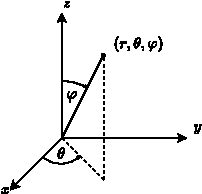
\includegraphics[width=\textwidth/2]{figures/background/spherical.pdf}
    \end{center}
    \caption[Spherical Coordinates]{Spherical Coordinates}
    \label{fig:spherical}
\end{figure}

where
\begin{conditions}
    r       & radial distance, $r \rightarrow \mathbb{R}$ \\
    \theta  & azimuthal angle, $\theta \rightarrow (-\pi, \pi]$ \\
    \varphi & polar angle, $\varphi \rightarrow [0, \pi]$
\end{conditions}

    \chapter{Simulation Models and General Approach}\label{chap:approach}
In this chapter the simulation models and their properties will be introduced.
These models will help to describe the physical effects used in the simulation.
The general simulation approach and an overview of ARTS will be presented and discussed in detail.

\section{Receiver and Source Model}\label{sec:receiverAndSource}
\textbf{3D Model}\newline
An acoustic source can be seen as a "speaker" and an acoustic receiver can be seen as a "microphone".
These two have common properties like a location, an orientation which defines their local coordinate system and a field-of-view (FOV) which represents their emission and reception characteristics depending on the outgoing/incoming angle. 
A good receiver FOV example is the human ear.
Turning your ear towards someone who is talking to you will improve the speech reception whereas turning away will decrease it.
We will assume that sources and receivers can be modeled by a single point $(x,y,z)$ in the 3D cartesian coordinate system.
This has been illustrated for the 2D case in \figref{fig:SourceReceiver} in a global coordinate system with $x$-axis and $y$-axis.
\begin{figure}[H]
    \begin{center}
    \subfloat[Receiver Model]{
        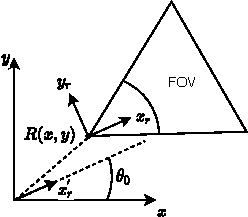
\includegraphics[width=\textwidth/2]{figures/approach/figReceiver.pdf}
    }
    \subfloat[Source Model]{
        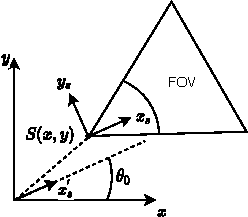
\includegraphics[width=\textwidth/2]{figures/approach/figSource.pdf}
    }
    \end{center}
    \caption[Source and Receiver Properties]{Source and Receiver Properties}
    \label{fig:SourceReceiver}
\end{figure}

Let's define the following conventions for the receiver
\begin{conditions}
    x, y, z         & Location in the global coordinate system \\
    x_r, y_r, z_r   & Local coordinate system with $x_r$-axis, $y_r$-axis and $z_r$-axis \\
    \theta_0        & azimuth angle between global $x$-axis and local $x_r$-axis \\
    \varphi_0       & polar angle between global $z$-axis and local $z_r$-axis
\end{conditions}
and accordingly for the source as well.
Additionally let's define a receiver FOV function 
\begin{equation}
    f_{FOV}(\theta_r, \varphi_r) \rightarrow [0, 1]
\end{equation}
for the reception characteristics and a source FOV function 
\begin{equation}
    g_{FOV}(\theta_s, \varphi_s) \rightarrow [0, 1]
\end{equation}
for the emission characteristics where the respective angles are relative to the local coordinate system.
In \figref{fig:fov} two simple examples are given and how a receiver characteristic could look like.
Evenly distributed (blue rectangle) for a radial receiver without any angle penalty $f(\theta, \varphi)=1$ or linearly decreasing when moving away from the center (red triangle).
The center of the receiver and source is defined by the respective $x_r$- and $x_s$-axis.
\begin{figure}[H]
    \begin{center}
    \subfloat[FOV for $\theta$]{
        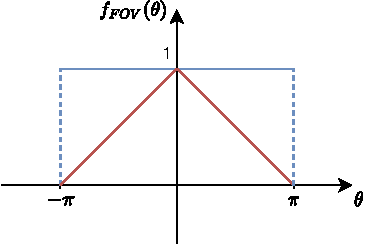
\includegraphics[width=\textwidth/2]{figures/approach/figFovTheta.pdf}
    }
    \subfloat[FOV for $\varphi$]{
        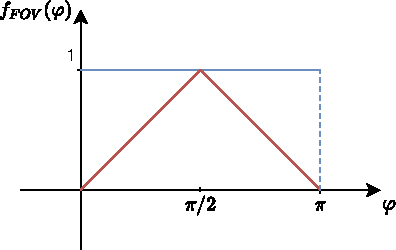
\includegraphics[width=\textwidth/2]{figures/approach/figFovPhi.pdf}
    }
    \end{center}
    \caption[FOV examples]{FOV examples}
    \label{fig:fov}
\end{figure}


\textbf{Receiver and Source Signals}\newline
Even though the geometry of receivers and sources is very similar, the signals are treated differently at the node positions.
A source signal is defined by
\begin{equation}
    s(t) = g_{FOV}(\theta_s, \varphi_s) \cdot x_s(t)
\end{equation}
for $t \in \mathbb{R}_0^+$ and a given direction $(\theta_s, \varphi_s)$ where
\begin{conditions}
    g_{FOV}(\theta_s, \varphi_s)    & Source FOV function \\
    x_s(t)                          & Continuous source signal function, $x_s(t) \rightarrow [-1,1]$ \\
    t                               & time in seconds $[s]$ 
\end{conditions}

The receiver signal on the other hand can be expressed as
\begin{equation}\label{approach:receiver}
    r[n] = f_{FOV}(\theta_r, \varphi_r) \cdot y(n \cdot T_r)
\end{equation}
for $n \in \mathbb{N}$ and a given direction $(\theta_r, \varphi_r)$ where
\begin{conditions}
    f_{FOV}(\theta_r, \varphi_r) & Receiver FOV function \\
    y_r(t) & Continuous receiver signal from direction $(\theta_r, \varphi_r)$, $y_r(t) \rightarrow \mathbb{R}$ \\
    T_r                          & Receiver Sampling Time, $T_r \in \mathbb{R}^+$ \\
    n                            & Sampling index
\end{conditions}

Note how the receiver signal is modeled as a discrete signal and not as a continuous signal.
This is a hint on how the signal is later going to be used.
A real world microphone does record continuously but the signal is later sampled at a given frequency in most systems.

\textbf{Definition}\newline
Given the introduced properties a source $S_i$ is defined by
\begin{itemize}
    \item a global coordinate $(x, y, z)$
    \item rotation $(\theta_0, \varphi_0)$ relative to global coordinate system
    \item output characteristic $g_{FOV}(\theta_s, \varphi_s)$
    \item a source signal $x_s(t)$
\end{itemize}
for $i \in {1,...,M}$ and a receiver $R_j$
\begin{itemize}
    \item a global coordinate $(x, y, z)$
    \item rotation $(\theta_0, \varphi_0)$ relative to global coordinate system
    \item input characteristic $f_{FOV}(\theta_r, \varphi_r)$
    \item sampling frequency $T_r$
\end{itemize}
for $j \in {1,...,N}$.

\section{Obstacle Model}\label{sec:obstacle}
In the model to be presented an "obstacle" is a surface that might reflect or absorb a sound wave.
Other suitable descriptions are "reflector" or "mirror". 
There are stationary obstacles, like walls, windows, doors, tables, TVs and furniture in general and mobile obstacles, like chairs, laptops, bottles and so on.

\textbf{3D Model}\newline
In this approach all types of obstacles are treated the same way and their geometry is defined by (2D-)Polygons with at least three points. If the points form a 2D-polygon they must define a plane $\Phi: ax + by + cz = d$ as well.

\begin{figure}[H]
    \begin{center}
    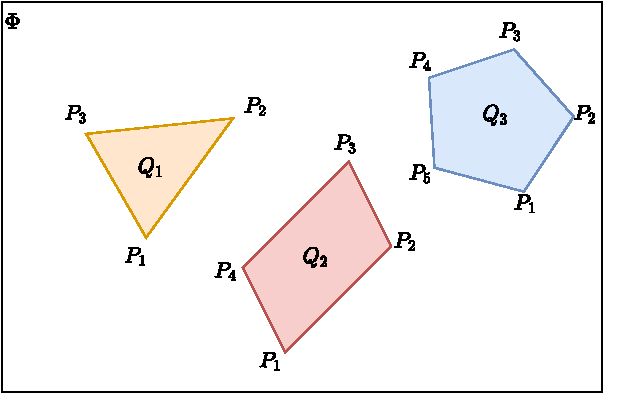
\includegraphics[width=\textwidth]{figures/approach/figObstacles.pdf}
    \end{center}
    \caption[Examples for Obstacles with $N=3,4,5$]{Examples for Obstacles with $N=3,4,5$}
    \label{fig:figObstacles}
\end{figure}


Therefore the geometry of an obstacle $Q_k$ is given by
\begin{itemize}
    \item a set of points $B_k = \{P_1(x,y,z), P_2(x,y,z), ..., P_N(x,y,z)\}$
    \item such that $B_k$ defines a plane $\Phi_k$
\end{itemize}
where $N \geq 3$.

\textbf{Specular Reflection}\newline
When we apply the "geometric acoustic" approach mentioned by Niklas Röber et al in \cite{rober2007ray} sound waves are approximated as particles moving along directional rays.
The reflection of these rays will be modeled the same way as in optics where the reflection angle $\alpha^{'}$ is equal to the incident angle $\alpha$ relative to the surface normal.
\begin{equation}
    \alpha^{'} = \alpha
\end{equation}
Additionally a reflection coefficient $\gamma_k \rightarrow [0,1]$ will be defined, which represents the relation between the outgoing ray intensity level $I_2$ and the incoming ray intensity $I_1$.
\begin{equation}
    \gamma_k = \frac{I_2}{I_1}
\end{equation}
\begin{figure}[H]
    \begin{center}
    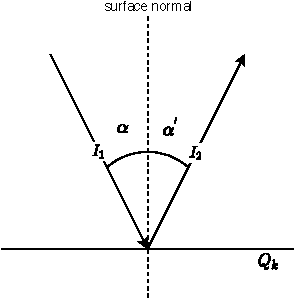
\includegraphics[width=\textwidth/2]{figures/approach/figSpecularReflection.pdf}
    \end{center}
    \caption[Specular reflection]{Specular reflection}
    \label{fig:specularReflection}
\end{figure}

\textbf{Other effects}\newline
As proposed in \cite{rober2007ray} wave phenomena such as "scattering", "diffraction" and the influence of the wavelength are worth mentioning but are usually discarded at higher frequencies.
Since we are looking into ultrasound ($f > 20\text{kHz}$) where the wavelength is much shorter than the dimensions of most obstacles this assumption will be applied for the scope of this thesis.
However these effects are still important for improving the reflection model and for noise generation and they should be introduced at some point.

\textbf{Definition}\newline
Given the discussed properties an obstacle $Q_k$ is defined by
\begin{itemize}
    \item a polygon of set $B_k$ of $N$ coplanar points lying on a plane $\Phi_k$
    \item a reflection coefficient $\gamma_k \rightarrow [0,1]$
\end{itemize}
where $N \geq 3$.

\section{Environment Model}\label{sec:environment}
In \secref{sec:backgroundBasic} we already defined an environment $E$, it is given by the tuple $(\vartheta, \phi, p)$ and a set $Q$ of $K$ obstacles.
The "simplest" environment therefore has no obstacles ($K=0$) and only relies on the temperature $\vartheta$, the relative humidity $\phi$ and atmospheric pressure $p$.
For the environment model these properties are assumed to be static and uniform across space for smaller indoor environments.
Their values will influence certain physical effects such as the speed of sound and mainly "path loss".

\textbf{Speed of sound}\newline
According to Reuben Thomas \cite{wayverb} speed of sound in air can be approximated by

\begin{equation}
    c_{\text{air}} = (331 + 0.6 \frac{\vartheta}{^{\circ}\textrm{C}})\frac{\text{m}}{\text{s}}
\end{equation}

\textbf{Path Loss}\newline
For spherical sound waves (point sources) the intensity in radial direction can be expressed as
\begin{equation}
    I(r) = \frac{P}{4 \cdot \pi \cdot r^2}\label{approach:intensity}
\end{equation}
where
\begin{conditions}
    P & sound power [W] \\
    r & sphere radius [m]
\end{conditions}
The relation $I(r) \propto 1/r^2$ is also referred to as the \textit{inverse-square law}.
Therefore we will approximate the damping of a source signal $s(t)$ by the following loss function
\begin{equation}
    \mathcal{L}(d) = \frac{1}{d+1}\label{approach:loss}
\end{equation}
where
\begin{conditions}
    d & distance travelled [m]
\end{conditions}
Friction and relaxation processes are another source for "path loss" and are described by Russel in \cite{drussell}.
Using Russel's absorption calculator and the values $\vartheta=20^{\circ}\textrm{C}, \phi=0\%, p=101\text{kPa}$ the result is $[6.53 \text{dB}/100\text{m}]$ for 20kHz and $[57.70 \text{dB}/100\text{m}]$ for 60kHz.
Russel shows that "air" can be described as a low-pass filter and that depending on the ultrasonic wave frequency the impact might be huge.
The current model however will for now only rely on the \eqref{approach:loss} as the loss function.

\newpage
\section{Approach Overview}
The general approach is to follow an architecture which is module based.
This will allow us to set clear boundaries for each type of problems while also allowing for optimizations to be made to each individual module independently.
For each module the input is clearly defined and usually results in a single output type which can then be fed to another module.
In the following sections each of these modules will be presented. 
An overview is given in \figref{fig:overview}.

\newpage
\begin{figure}[H]
    \begin{center}
    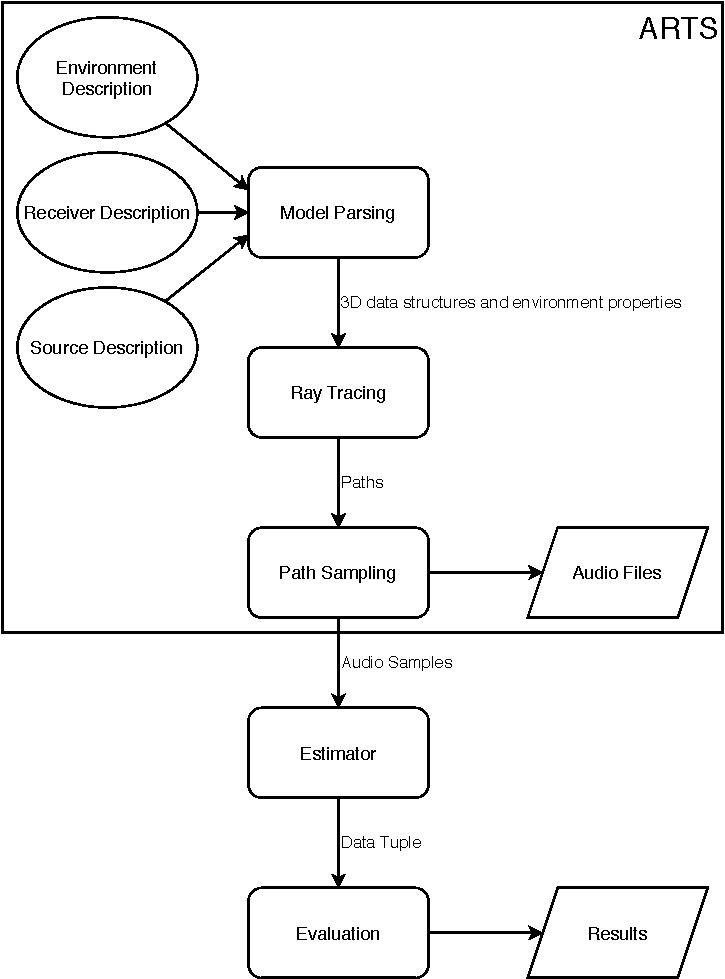
\includegraphics[width=\textwidth]{figures/approach/figOverview.pdf}
    \end{center}
    \caption[Acoustic Ray Tracing Simulator overview]{Acoustic Ray Tracing Simulator overview}
    \label{fig:overview}
\end{figure}

 
\section{Model Parsing}
The Model Parser is the first module of the pursued approach.
It is important that all the properties of a setup $A$ can be loaded in the simulation.
We are dealing mainly with 3D data combined with some physical properties, see \secref{sec:receiverAndSource}, \secref{sec:obstacle} and \secref{sec:environment}.
Therefore a suitable description for these models should be chosen.
The generated 3D data structures and environmental properties will then be used in the following modules.

\begin{figure}[H]
    \begin{center}
    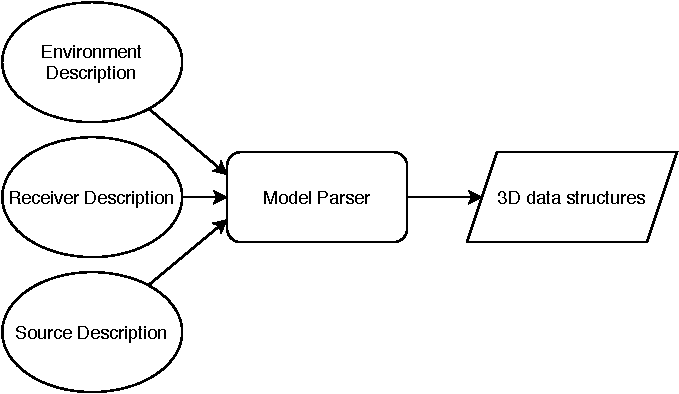
\includegraphics[width=\textwidth]{figures/approach/figModelParser.pdf}
    \end{center}
    \caption[Model Parsing]{Model Parsing}
    \label{fig:modelParser}
\end{figure}


\section{Ray Tracing}
The 3D data structures should represent the sources, receivers and obstacles in a way that simple geometrical operations can be performed, such as "point mirroring", "intersection of rays and obstacles", "distance calculation between points" and so on.
The Ray Tracer should only deal with the geometrical problem of finding paths between sources and receivers.
\begin{figure}[H]
    \begin{center}
    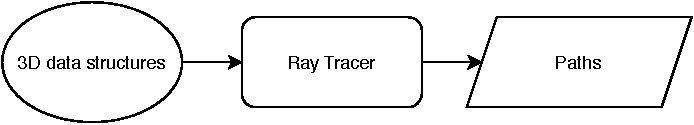
\includegraphics[width=\textwidth]{figures/approach/figRayTracer.pdf}
    \end{center}
    \caption[Ray Tracer Module]{Ray Tracer Module}
    \label{fig:rayTracer}
\end{figure}

The problem to be solved can be stated relatively simple.
For each pair $(S_i, R_j)$, one source $S_i$ and one receiver $R_j$, all possible geometric paths need to be found in an Environment $E$ with $K$ obstacles.

Reflections will be categorized by an Order $L \in \mathbb{N}$. 
They will be referenced as "reflections of order $L$".
The order $L$ tells us how often the ray bounces around until it reaches the receiver $R_j$.
As an example, the special case for $L=0$ is called "direct path" and does not bounce at all.

A Segment $A$ is defined by two locations $A_1(x,y,z)$ and $A_2(x,y,z)$ and a Path $P_{ij}$ is defined by concatenating a sequence of segments, where the starting point is a source $S_i$ and the end point is a source $R_j$. A path can therefore be expressed as

\begin{equation}
    P_{ij} = \{ S_i \rightarrow A_1 \rightarrow A_2 \rightarrow ... \rightarrow A_L \rightarrow R_j\} 
\end{equation}

Let's start with simple examples to figure out the conditions that a source $S_i$ can actually reach the receiver $R_j$.

\textbf{First Condition: No collisions}\newline
A path can only exist if every segment contained does not collide with any obstacle $Q_i$.
Take a look at \figref{fig:collision} for the direct path scenario.
\begin{figure}[H]
    \begin{center}
    \subfloat[Collision-free]{
        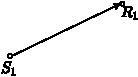
\includegraphics[width=0.5\textwidth]{figures/approach/figNoCollision.pdf}
    }
    \subfloat[Collision detected]{
        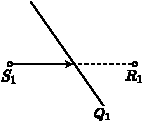
\includegraphics[width=0.5\textwidth]{figures/approach/figCollision.pdf}
    }
    \end{center}
    \caption[Collision cases]{Collision cases}
    \label{fig:collision}
\end{figure}

This condition is true for reflections as well, which consist of $L+1$ Segments.
If the segment starts or ends at a reflection point, the according obstacle should be excluded from this condition.

\textbf{Second Condition: Reflection point exists}\newline
In this example the first order reflection will be considered. 
To ensure that a reflection actually exists two operations need to be performed:
\begin{itemize}
    \item Mirror the receiver point $R_1$ at plane $\Phi_1$ to get the mirroring point $H_1$
    \item Check if segment $(S_1, H_1)$ intersects with the obstacle $Q_1$ in $I_1$
\end{itemize}
\begin{figure}[H]
    \begin{center}
    \subfloat[Reflection of first order]{
        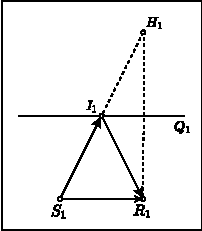
\includegraphics[width=0.5\textwidth]{figures/approach/figReflection.pdf}
    }
    \subfloat[No reflection (intersection point $I_1$ does not exist)]{
        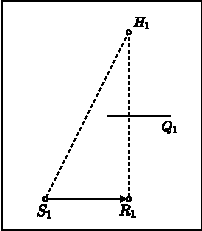
\includegraphics[width=0.5\textwidth]{figures/approach/figNoReflection.pdf}
    }
    \end{center}
    \caption[Reflection cases]{Reflection cases}
    \label{fig:reflection}
\end{figure}

Same as before, this check must hold for higher order reflections as well.

\textbf{Higher order reflections}\newline
For higher order reflections another notation is necessary to distinguish all possible paths and its members.
The previous notation might be enough for first order reflections but a more general description is needed for higher order reflections.
Let $T_l$ be a bounce tuple of length $l \in \{1,...,L\}$ describing a possible obstacle "bounce path".

\begin{itemize}
    \item For first order reflections $L = 1, T_1 = (k_1)$
    \item For second order reflections $L = 2, T_2 = (k_1, k_2)$
    \item For third order reflections $L = 3, T_3 = (k_1, k_2, k_3)$
\end{itemize}
where $k_p \in \{1,...,K\}$ such that $k_{p} \neq k_{p-1}$ for $L > 1$.

A bounce tuple only describes which obstacles $Q_k$ are being visited whereas a regular path describes the sequence of exact locations.
These exact locations for a given tuple $T_l$ are called reflection/intersection point $I_p^{T_l}$ for $p \in \{1,...,L\}$.
In order to get and construct these points the mirrored points $H_p^{T_l}$ for $p \in \{1,...,L\}$ of a receiver $R_j$ are needed.
The existence of these reflection points $I_p^{T_l}$ needs to be confirmed first as we know from the second condition.
An illustration of the notation is given by the example in \figref{fig:higherOrder}.
\begin{figure}[H]
    \begin{center}
    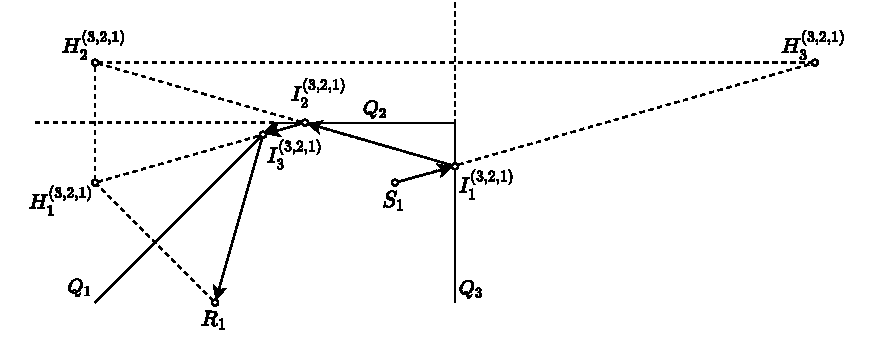
\includegraphics[width=\textwidth]{figures/approach/figHigherOrder.pdf}
    \end{center}
    \caption[$L=3$, Third order example with new notation]{$L=3$, Third order example with new notation}
    \label{fig:higherOrder}
\end{figure}


To summarize the different types of paths:
\begin{itemize}
    \item Direct Path $P_{ij} = \{ S_i \rightarrow R_j \}$
    \item First order path $P_{ij}^{T_1} = \{ S_i \rightarrow I_1^{T_1} \rightarrow R_j \}$
    \item Second order path $P_{ij}^{T_2} = \{ S_i \rightarrow I_1^{T_2} \rightarrow I_2^{T_2}\rightarrow R_j \}$
    \item Third order path $P_{ij}^{T_3} = \{ S_i \rightarrow I_1^{T_3} \rightarrow I_2^{T_3} \rightarrow I_3^{T_3} \rightarrow R_j \}$
\end{itemize}

\textbf{Graphs}\newline
Since the goal is to get all the existing paths for a pair $(S_i, R_j)$ a graph $G_{ij}$ can be described as $G_{ij} = \{P_{ij}\} \cup \{P_{ij}^{T_1}\} \cup \{P_{ij}^{T_2}\} \cup \{P_{ij}^{T_3}\}$ for all existing bounce paths $T_1$, $T_2$, and $T_3$.
An illustration for a "full graph" $G_{ij}$ is given in \figref{fig:graph} for $K=2$ and $L=3$.
\begin{figure}[H]
    \begin{center}
    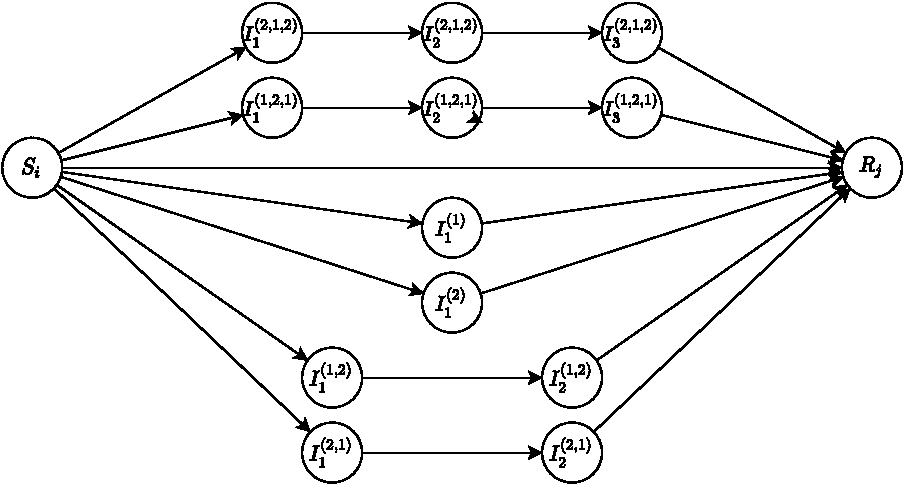
\includegraphics[width=\textwidth]{figures/approach/figGraph.pdf}
    \end{center}
    \caption[Full graph example for $K=2$ and $L=3$]{Full graph example for $K=2$ and $L=3$}
    \label{fig:graph}
\end{figure}


\textbf{Strategy Summary}\newline
For each possible path we need to perform the following actions:
\begin{enumerate}
    \item Mirroring $R_j$ backwards to get mirroring points $H_p^{T_l}$ for $p \in \{1,...,L\}$
    \item Travelling forward to get intersection points $I_p^{T_l}$
    \begin{itemize}
        \item Check if reflection point $I_p^{T_l}$ exists
        \item Check if new segment collides with other obstacles
        \item Add segments to path until $R_j$ is reached
    \end{itemize}
\end{enumerate}

\textbf{Run-time Complexity}\newline
Given that the current strategy is performed on all possible paths the following complexity $C_l$ for a specific order $l > 0, l \in \{1,...,L\}$ can be expected:
\begin{equation}
    C_l = M \cdot N \cdot K \cdot (K-1)^{l-1}
\end{equation}
where
\begin{conditions}
    M & The number of sources $S_i$ \\
    N & The number of receivers $R_j$ \\
    K & The number of obstacles $Q_k$
\end{conditions}

The total number of paths and the total complexity $C_L$ for all full graphs $G_{ij}$ can be expressed as
\begin{equation}\label{eq:complex}
    C_L = M \cdot N + \sum_{l=1}^{L}{C_l} =  M \cdot N \cdot ( 1 + K \cdot \sum_{l=1}^{L}{(K-1)^{l-1}})
\end{equation}

This sets an upper bound for the complexity of the current strategy.
A lot of paths will probably fail to satisfy one of the two checks and therefore terminate earlier.
The first step however is performed for every possible path, therefore run-times of order $C_L$ are expected.

\section{Path Sampling}
The "Ray Tracer" provides a set of paths in form of a Graph $G_{ij}$.
Each path might contribute to the final received signal depending on the properties of a path $P$ in $G_{ij}$ and the environmental properties introduced in the previous chapters.
The "Path Sampler" takes all these modeled effects and creates a set of samples for each $(S_i, R_j)$ pair.

\begin{figure}[H]
    \begin{center}
    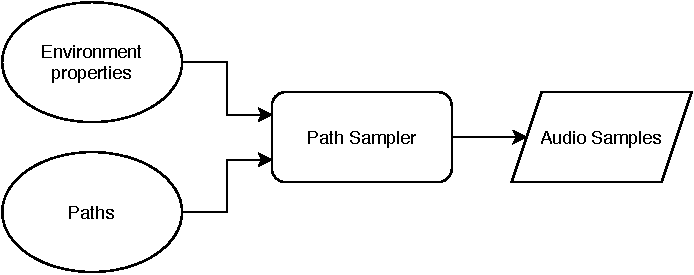
\includegraphics[width=\textwidth]{figures/approach/figPathSampler.pdf}
    \end{center}
    \caption[Path Sampler Module]{Path Sampler Module}
    \label{fig:pathSampler}
\end{figure}

In \eqref{approach:receiver} a first sneak peek was given on how an incoming signal $r[n]$ will be sampled.
A lot of different models have been introduced since then and they will now be condensed into a single equation for the total received signal $r_{ij}[n]$:
\begin{equation}\label{eq:receiver}
    r_{ij}[n] = \sum_{P \in G_{ij}} f_{FOV}(\theta_{r,P}, \varphi_{r,P}) \cdot \mathcal{L}(d_P) \cdot \prod_{\gamma_k \in P}{\gamma_k} \cdot g_{FOV}(\theta_{s,P}, \varphi_{s,P}) \cdot x_s(n \cdot T_r - \frac{d_P}{c_{\text{air}}})
\end{equation}
where
\begin{conditions}
    P & Path in Graph $G_{ij}$ \\
    d_P & Total Path length of $P$ in [m] \\
    f_{FOV}(\theta_{r,P}, \varphi_{r,P}) & Receiver $R_j$ FOV factor for incoming direction of path $P$ \\
    \mathcal{L}(d_P) & Distance $d_P$ loss factor \\
    \prod_{\gamma_k \in P}{\gamma_k} & Combined Reflection factor for all obstacles $Q_k$ in $P$ \\
    g_{FOV}(\theta_{s,P}, \varphi_{s,P}) & Source $S_i$ FOV factor for outgoing direction of path $P$ \\
    x_s(t) & Source signal of $S_i$ \\
    n  & Sampling index \\
    T_r & Receiver $R_j$ sampling time in [s] \\
    c_{\text{air}} & Speed of sound in [m/s]
\end{conditions}

\section{Estimation and Evaluation}
An estimator represents a system that is trying to solve a certain problem.
Indoor localization estimators will most likely try to estimate locations $(x,y,z)$ in the room like in \cite{bordoy2019exploiting}, angle of arrivals (AOA) $(\theta, \varphi)$, time difference of arrival (TDOA) $(t_1, t_2,...)$ and so on.

Indoor mapping applications will try to estimate the room geometry.
This can be expressed as a tuple of normal vectors $(\vec{n_1},\vec{n_2},...)$ for distances to walls and obstacles similar to \cite{ribeiro2011geometrically} or in the best case 3D data structures of the environment.

Another example could be that the simulator should be improved.
Therefore the estimation process can be skipped completely, acting as a pass-through.
This could be very useful for optimizing the simulator using real world recordings.

Since the nature, the algorithms and the approaches of these systems vary a lot, this part has been left open to be generalized. In \chapref{chap:experiments} an example will be shown for a LOS localization estimator.

\begin{figure}[H]
    \begin{center}
    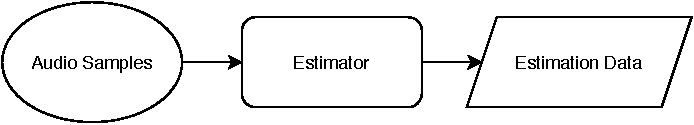
\includegraphics[width=\textwidth]{figures/approach/figEstimator.pdf}
    \end{center}
    \caption[Estimator Module]{Estimator Module}
    \label{fig:estimator}
\end{figure}


The evaluation of a system is highly coupled to the estimator.
Therefore it is up to the estimator to provide a suitable evaluation.
A well established error measure for vectors in general is the euclidean distance of two vectors
\begin{equation}
    \lVert \mathbf{\widetilde{x} - \mathbf{x}} \rVert_2 = \sqrt{(\tilde{x_1}-x_1)^2 + (\tilde{x_2}-x_2)^2 + ... + (\tilde{x_n}-x_n)^2}
\end{equation}
where
\begin{conditions}
    \mathbf{\widetilde{x}} & Estimation vector with length $n$ \\
    \mathbf{x} & True value vector with length $n$ \\
\end{conditions}
In the Evaluator Model the estimated values would be represented by $\mathbf{\widetilde{x}}$ and the real properties of the 3D data vectors by $\mathbf{x}$.
This approach will be used for the LOS localization estimator example in \chapref{chap:experiments}.
For non-vector types other approaches should be defined.

\begin{figure}[H]
    \begin{center}
    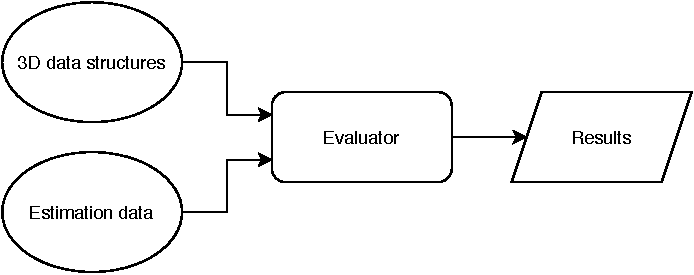
\includegraphics[width=\textwidth]{figures/approach/figEvaluator.pdf}
    \end{center}
    \caption[Evaluator Module]{Evaluator Module}
    \label{fig:evaluator}
\end{figure}


    \chapter{Acoustic Ray Tracing Simulator (ARTS)}\label{chap:experiments}
In this chapter the implementation of the presented methods in \chapref{chap:approach} will be introduced and how ARTS can be used for a simple LOS (line of sight) localization algorithm using multilateration.
Furthermore the run times of the mentioned modules "Ray Tracer" and "Path Sampler" in the previous chapter will be presented and discussed.\newline
The source code for ARTS can be found on \url{https://github.com/mguc/arts}.
Use the README to get started.
All the references made in this chapter are based on \textbf{v1.0.0} of ARTS and a tag with that version can be found on the repository.

All tests have been performed on a system with an Intel Core i9-8950HK CPU @ 2.90GHz.

\newpage
\section{Setup Data}
There were mainly three environments used for testing:

1. A room called "reference room" which features a cuboid representing a 4m x 5m x 3m room. The origin $(0,0,0)$ is located in the center of the room.
\begin{figure}[H]
    \begin{center}
    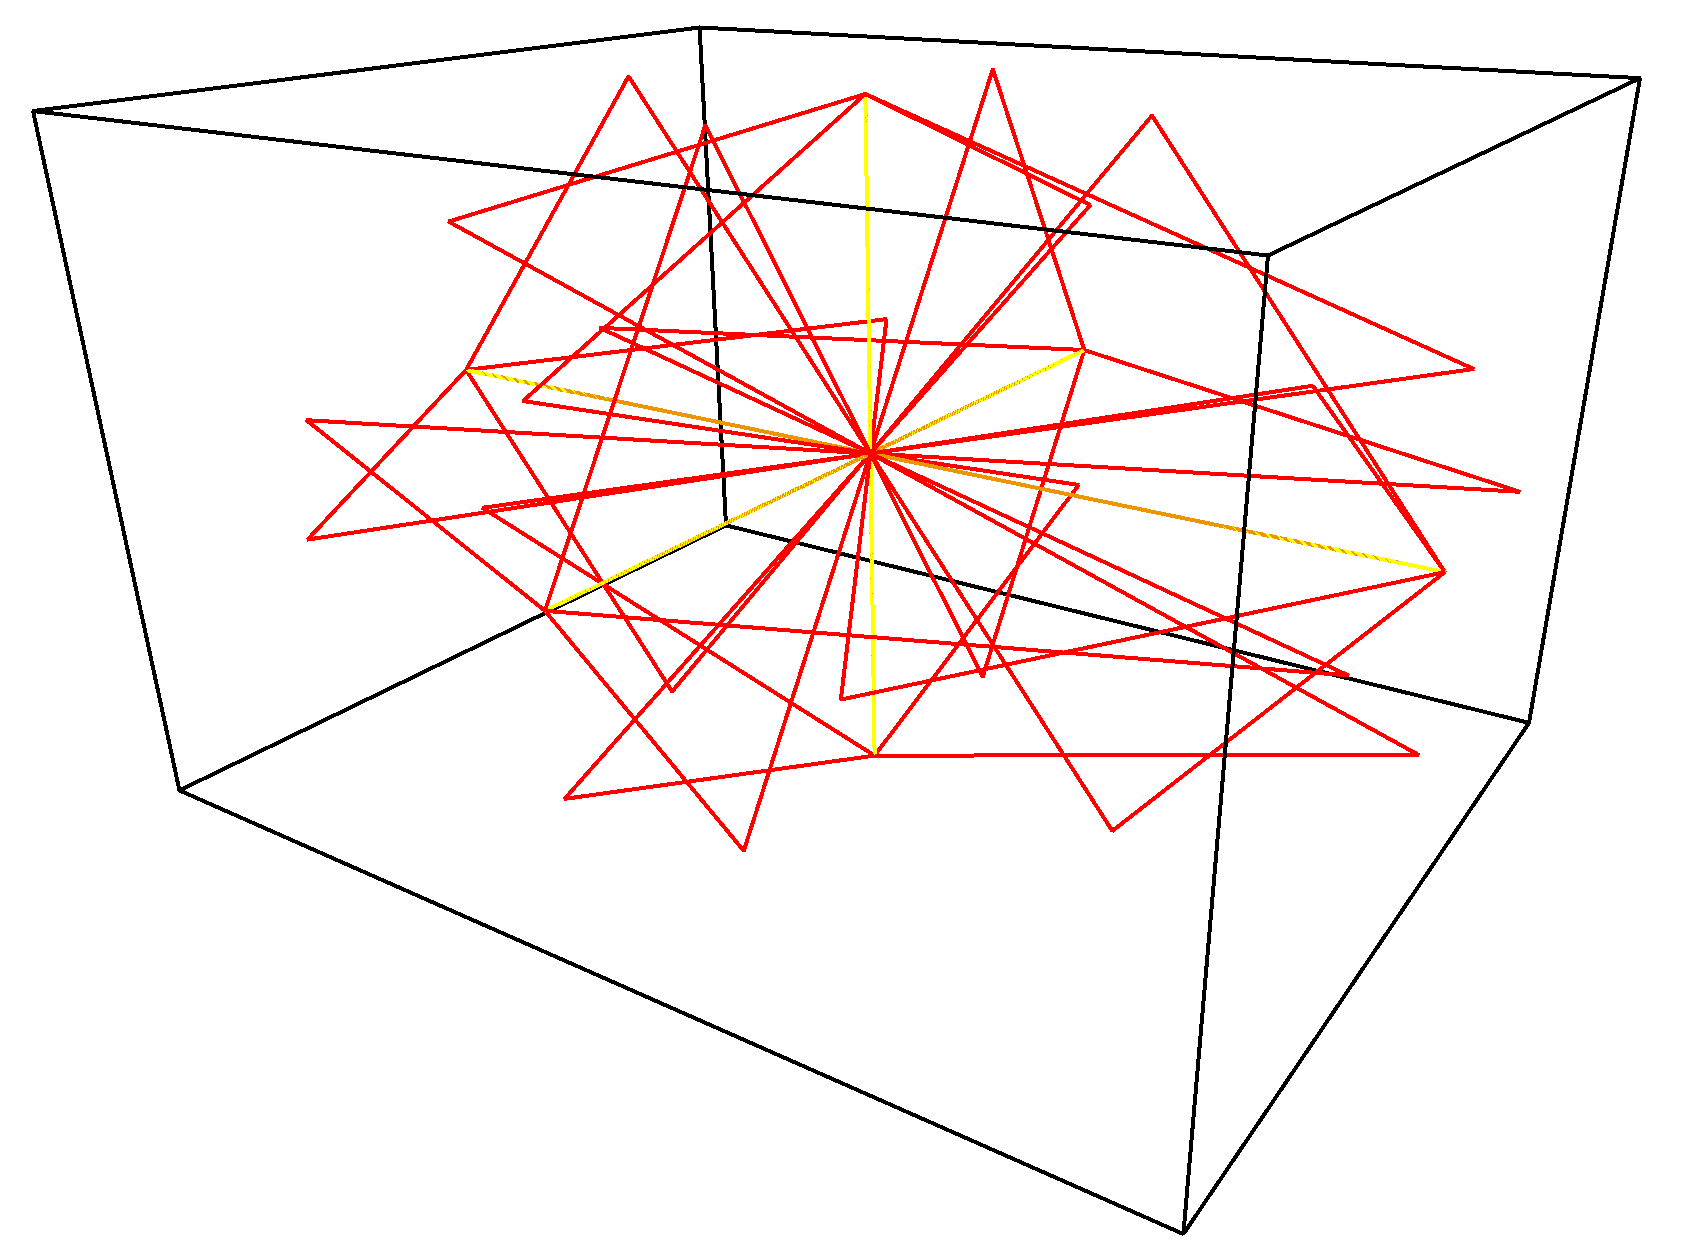
\includegraphics[width=\textwidth]{figures/experiments/reference_room.png}
    \end{center}
    \caption[Reference Room 4m x 5m x 3m]{Reference Room 4m x 5m x 3m}
    \label{fig:referenceRoom}
\end{figure}

\newpage
2. The "Tube", which only contains a "floor" and a "ceiling". Floor and ceiling are 1m apart and have a surface area of 2m x 2m. It looks like a tube in $x$-$z$ or $y$-$z$ view, therefore the name.
\begin{figure}[H]
    \begin{center}
    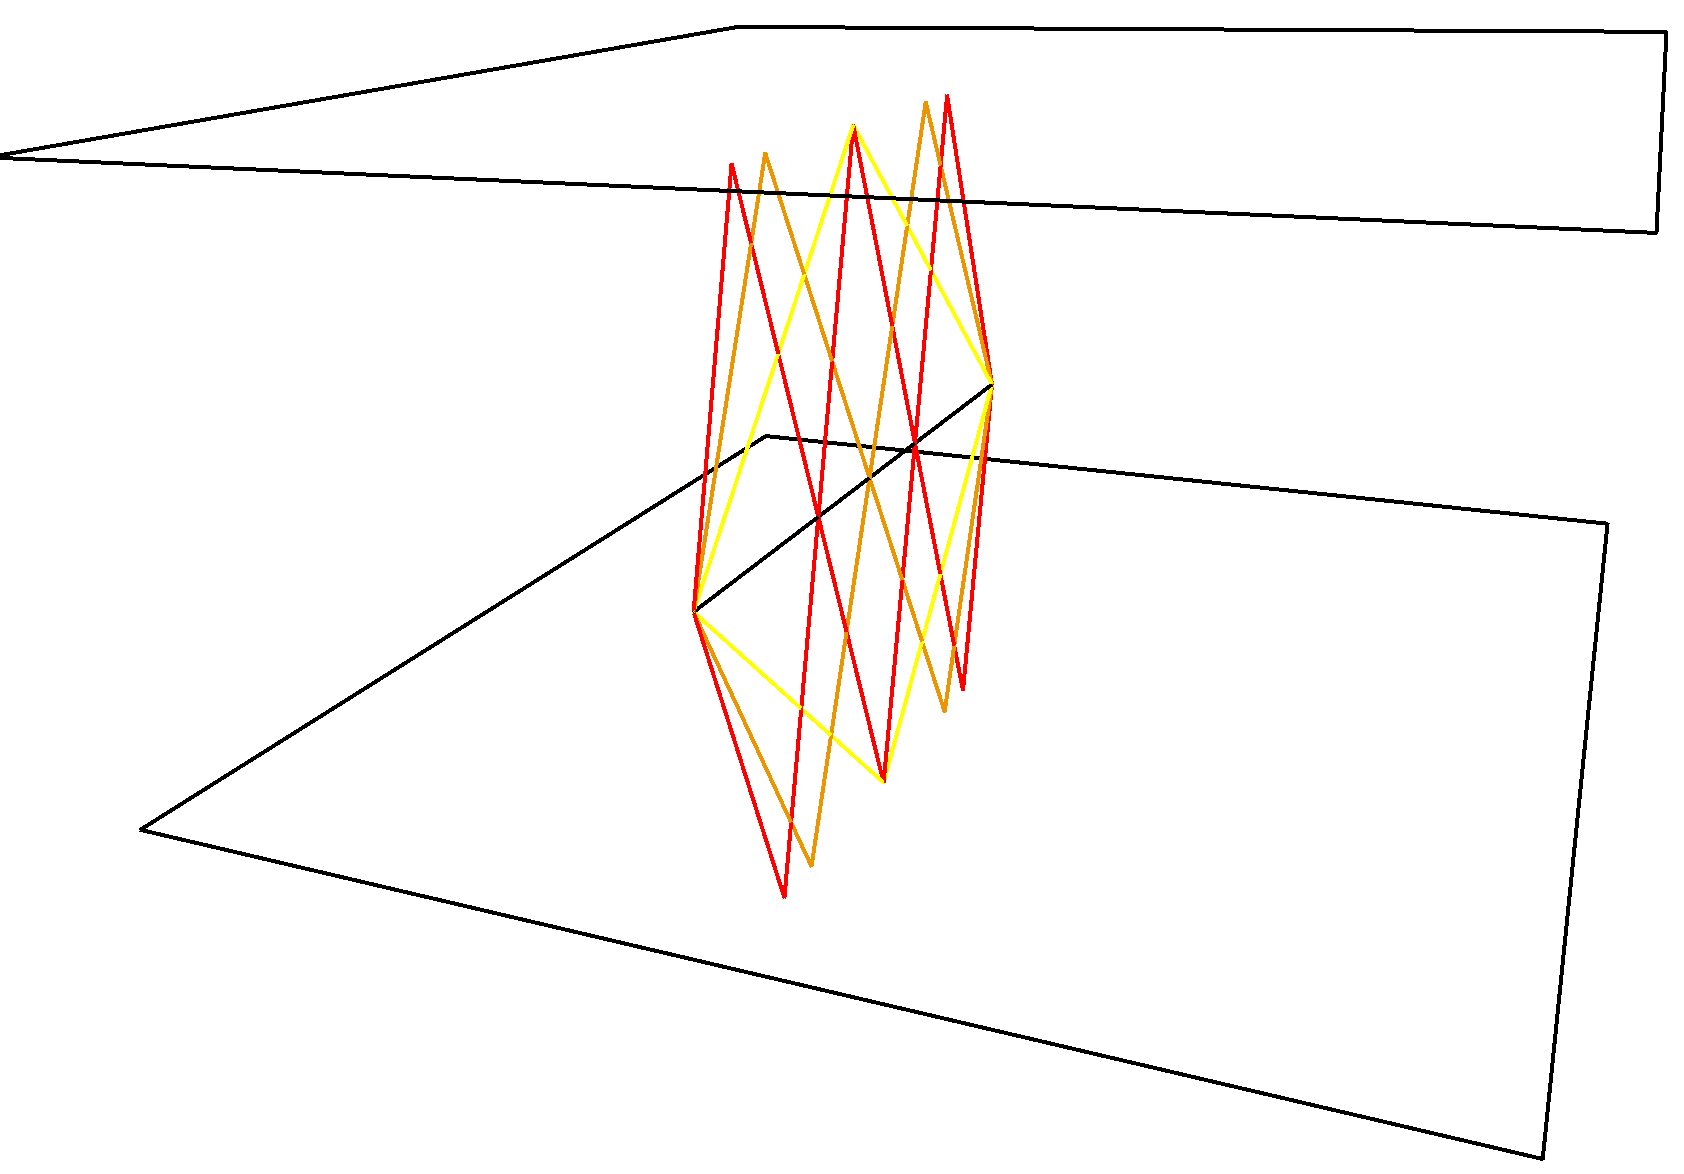
\includegraphics[width=\textwidth]{figures/experiments/tube_100.png}
    \end{center}
    \caption[Tube with Source at $(1,0,0)$ and Receiver at $(0,0,0)$]{Tube with Source at $(1,0,0)$ and Receiver at $(0,0,0)$}
    \label{fig:tube}
\end{figure}

\newpage
"Matryoshka Cube" which consists of $X$ nested cubes representing an environment with $6X$ obstacles $Q_1 ... Q_{6X}$.
\begin{figure}[H]
    \begin{center}
    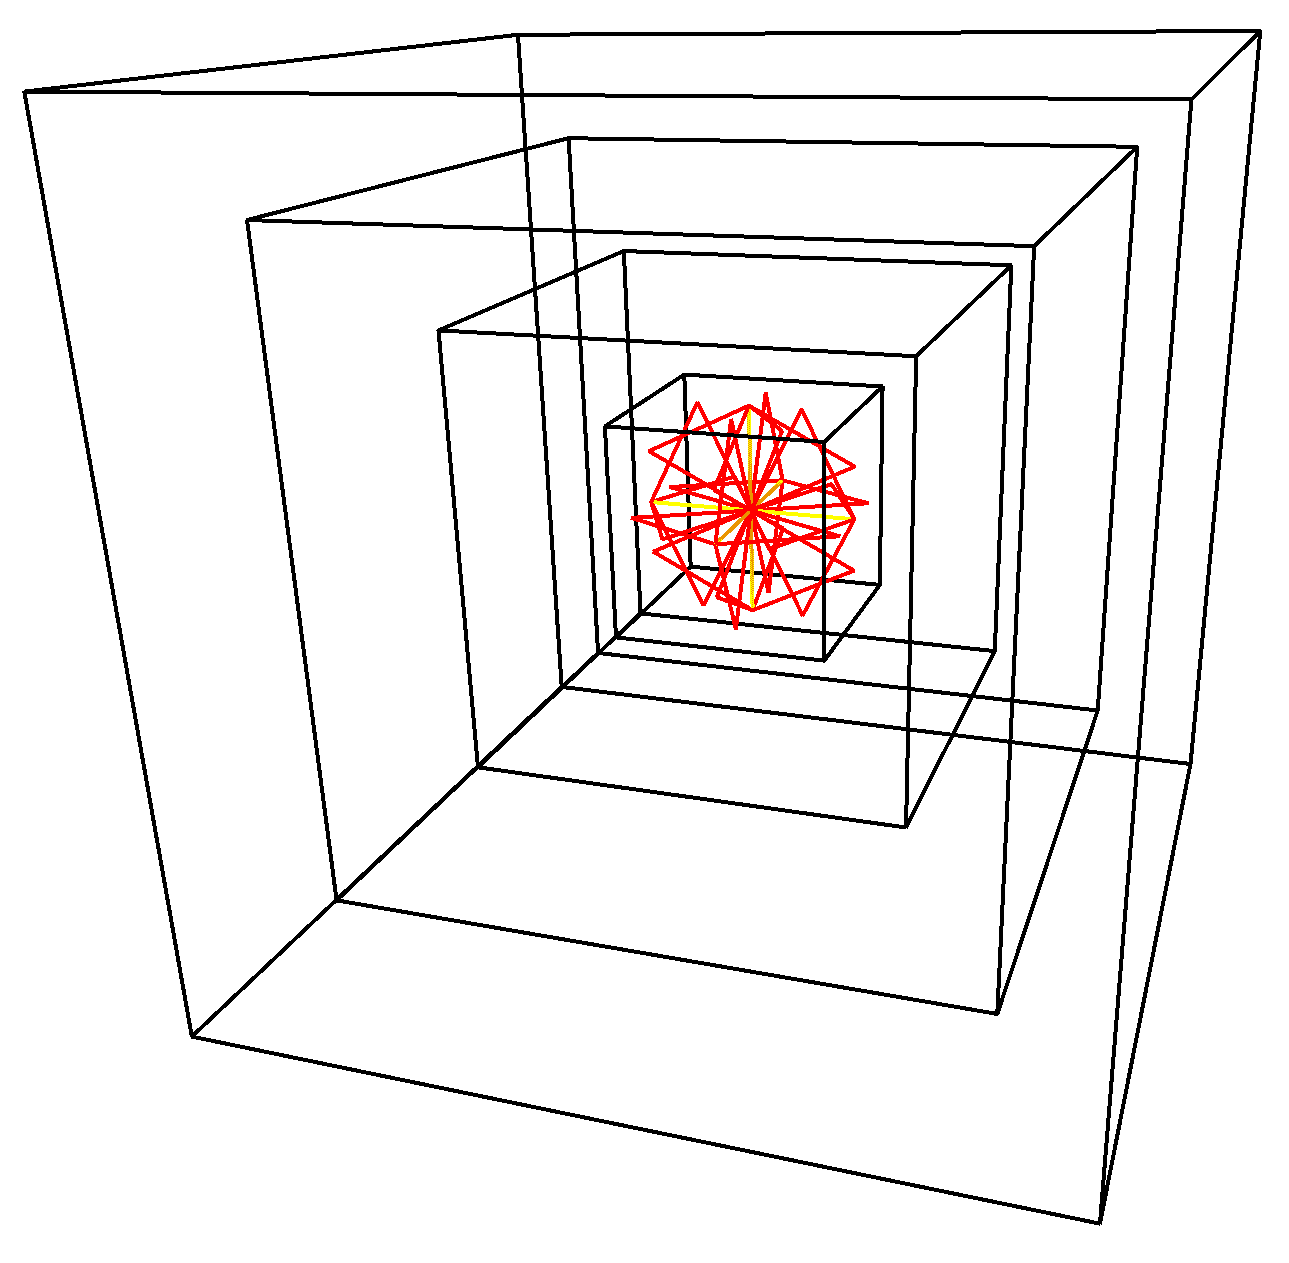
\includegraphics[width=\textwidth]{figures/experiments/matryoshka_4.png}
    \end{center}
    \caption[Matryoshka Cube with $X=4$ nested cubes]{Matryoshka Cube with $X=4$ nested cubes}
    \label{fig:matryoshka4}
\end{figure}


\newpage
\section{Model Simplification}\label{sec:modelSimplification}
In \textbf{v1.0.0} of ARTS not all features and properties discussed in the previous \chapref{chap:approach} have been implemented.\newline
Obstacles $Q_k$ will be treated as "perfect" reflectors, resulting in a reflection coefficient $\gamma_k = 1$ for all $k \in \{1,...,K\}$.
Receivers and Sources will use a rectangular FOV function resulting in $f_{FOV}(\theta_r, \varphi_r) = 1$ and $g_{FOV}(\theta_s, \varphi_s) = 1$.
This simplifies \eqref{eq:receiver} and results in the following receiver sampling equation:
\begin{equation}
    r_{ij}[n] = \sum_{P \in G_{ij}} \mathcal{L}(d_P) \cdot x_s(n \cdot T_r - \frac{d_P}{c_{\text{air}}})
\end{equation}
For $x_s(t)$ a slightly modified unit sample function $\delta[n]$ will be used, see \figref{fig:delta}.
The width of the pulse will be extended to match the sampling width $T_r$ of the receivers.
The pulse width of $\delta[n]$ will be extended such that $T_p < T_r$.
This will ensure that the pulse is seen by the receiver exactly once.
The sampling frequency for the receivers is set to 1MHz therefore resulting in a sampling width of $T_r = 10^{-6}\text{s}$.
\begin{figure}[H]
    \begin{center}
    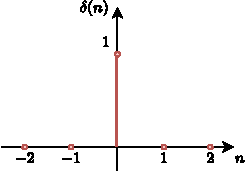
\includegraphics[width=0.5\textwidth]{figures/experiments/figDelta.pdf}
    \end{center}
    \caption[Unit sample function $\delta(n)$]{Unit sample function $\delta(n)$}
    \label{fig:delta}
\end{figure}

One big advantage of this approach is that the "room impulse response" (RIR) for a source location can be obtained.
The RIR will represent the travel time for the existing paths $P \in G_{ij}$.
This also means that a potential signal pre-processing can be skipped for estimators. In \figref{fig:RIR} the RIR for the reference room can be seen for a receiver and source sitting at the same location $(0,0,0)$.
\begin{figure}[H]
    \begin{center}
    \subfloat[RIR for $L=1$]{
        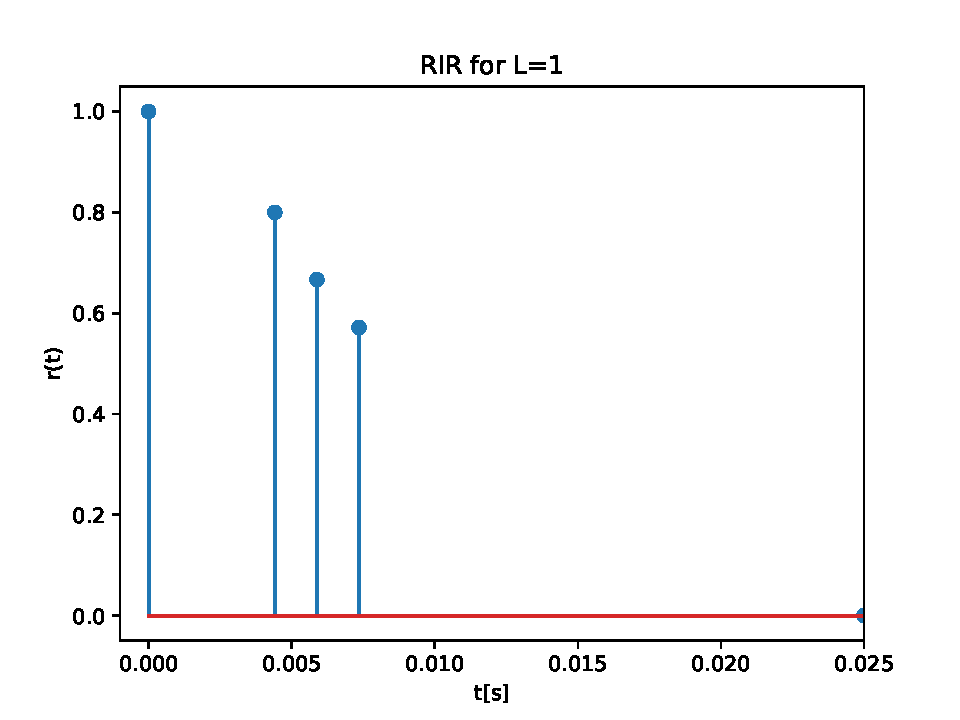
\includegraphics[width=\textwidth/2]{figures/experiments/rir1.pdf}
    }
    \subfloat[RIR for $L=2$]{
        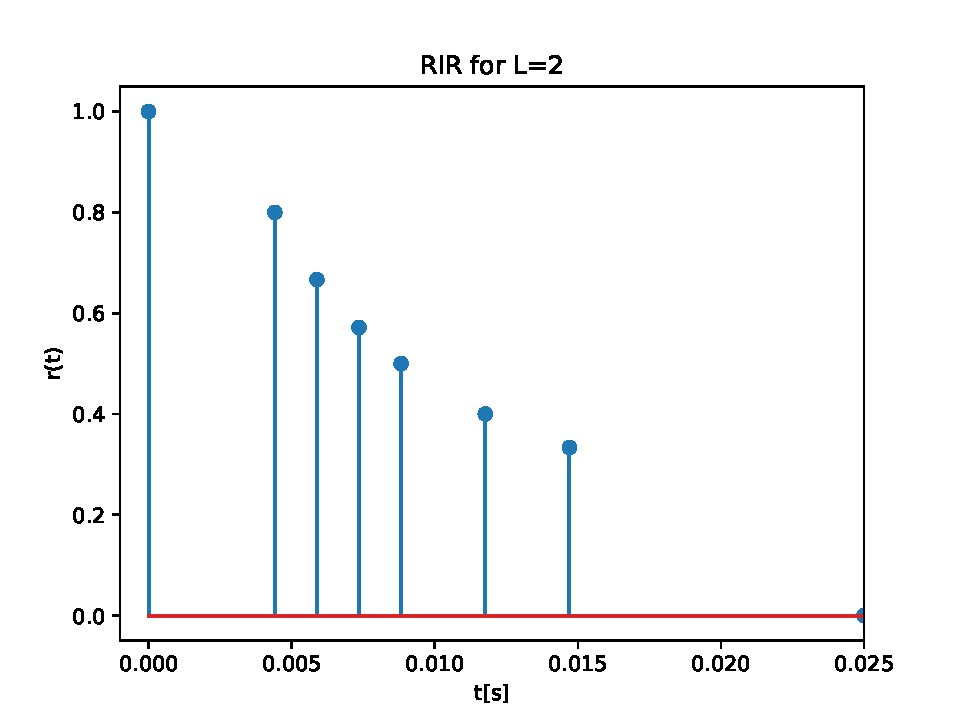
\includegraphics[width=\textwidth/2]{figures/experiments/rir2.pdf}
    }\\
    \subfloat[RIR for $L=3$]{
        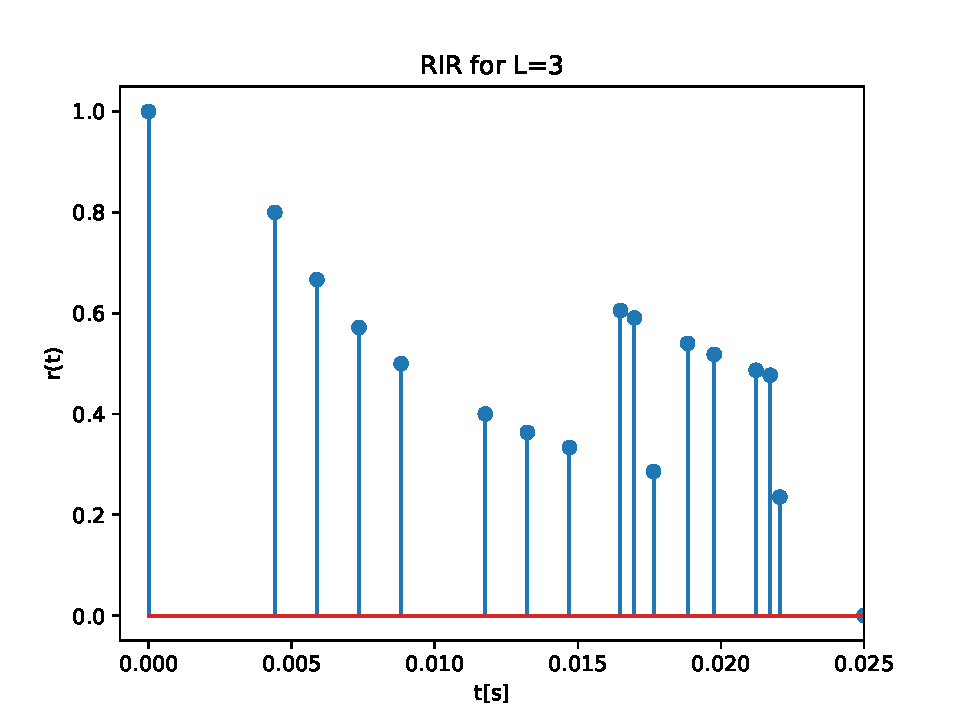
\includegraphics[width=\textwidth]{figures/experiments/rir3.pdf}
    }
    \end{center}
    \caption[Reference Room RIR]{Reference Room RIR}
    \label{fig:RIR}
\end{figure}


\section{ARTS Input Data}
In the ARTS repository the input data is located in the resource folder "rsc" and split by type: environment, receiver and source.

\textbf{Obstacles $Q_k$}\newline
The "Wavefront .obj file" format \cite{mreddy} will be used to represent the environment geometry and its obstacles $Q_k$. 
It is a format which is human readable and easy to comprehend. 
Most 3D modelling tools support the OBJ format and therefore make it a suitable candidate to define rooms and obstacles. 
This is a snippet for the reference room exported from Blender \cite{blender}:
\begin{verbatim}
    # Blender v2.79 (sub 0) OBJ File: '4x5x3room.blend'
    # www.blender.org
    mtllib 4x5x3room.mtl
    o Cube
    v 2.0 2.5 -1.5
    v 2.0 -2.5 -1.5
    v -2.0 -2.5 -1.5
    v -2.0 2.5 -1.5
    v 2.0 2.5 1.5
    v 2.0 -2.5 1.5
    v -2.0 -2.5 1.5
    v -2.0 2.5 1.5
    ...
    f 1//1 2//1 3//1 4//1
    f 5//2 8//2 7//2 6//2
    f 1//3 5//3 6//3 2//3
    f 2//4 6//4 7//4 3//4
    f 3//5 7//5 8//5 4//5
    f 5//6 1//6 4//6 8//6
\end{verbatim}

A line with a "v" represents a vertex (point in 3D) and "f" defines a face with vertex indices.
In \figref{fig:house} a more advanced 3D model is shown.
\begin{figure}[H]
    \begin{center}
    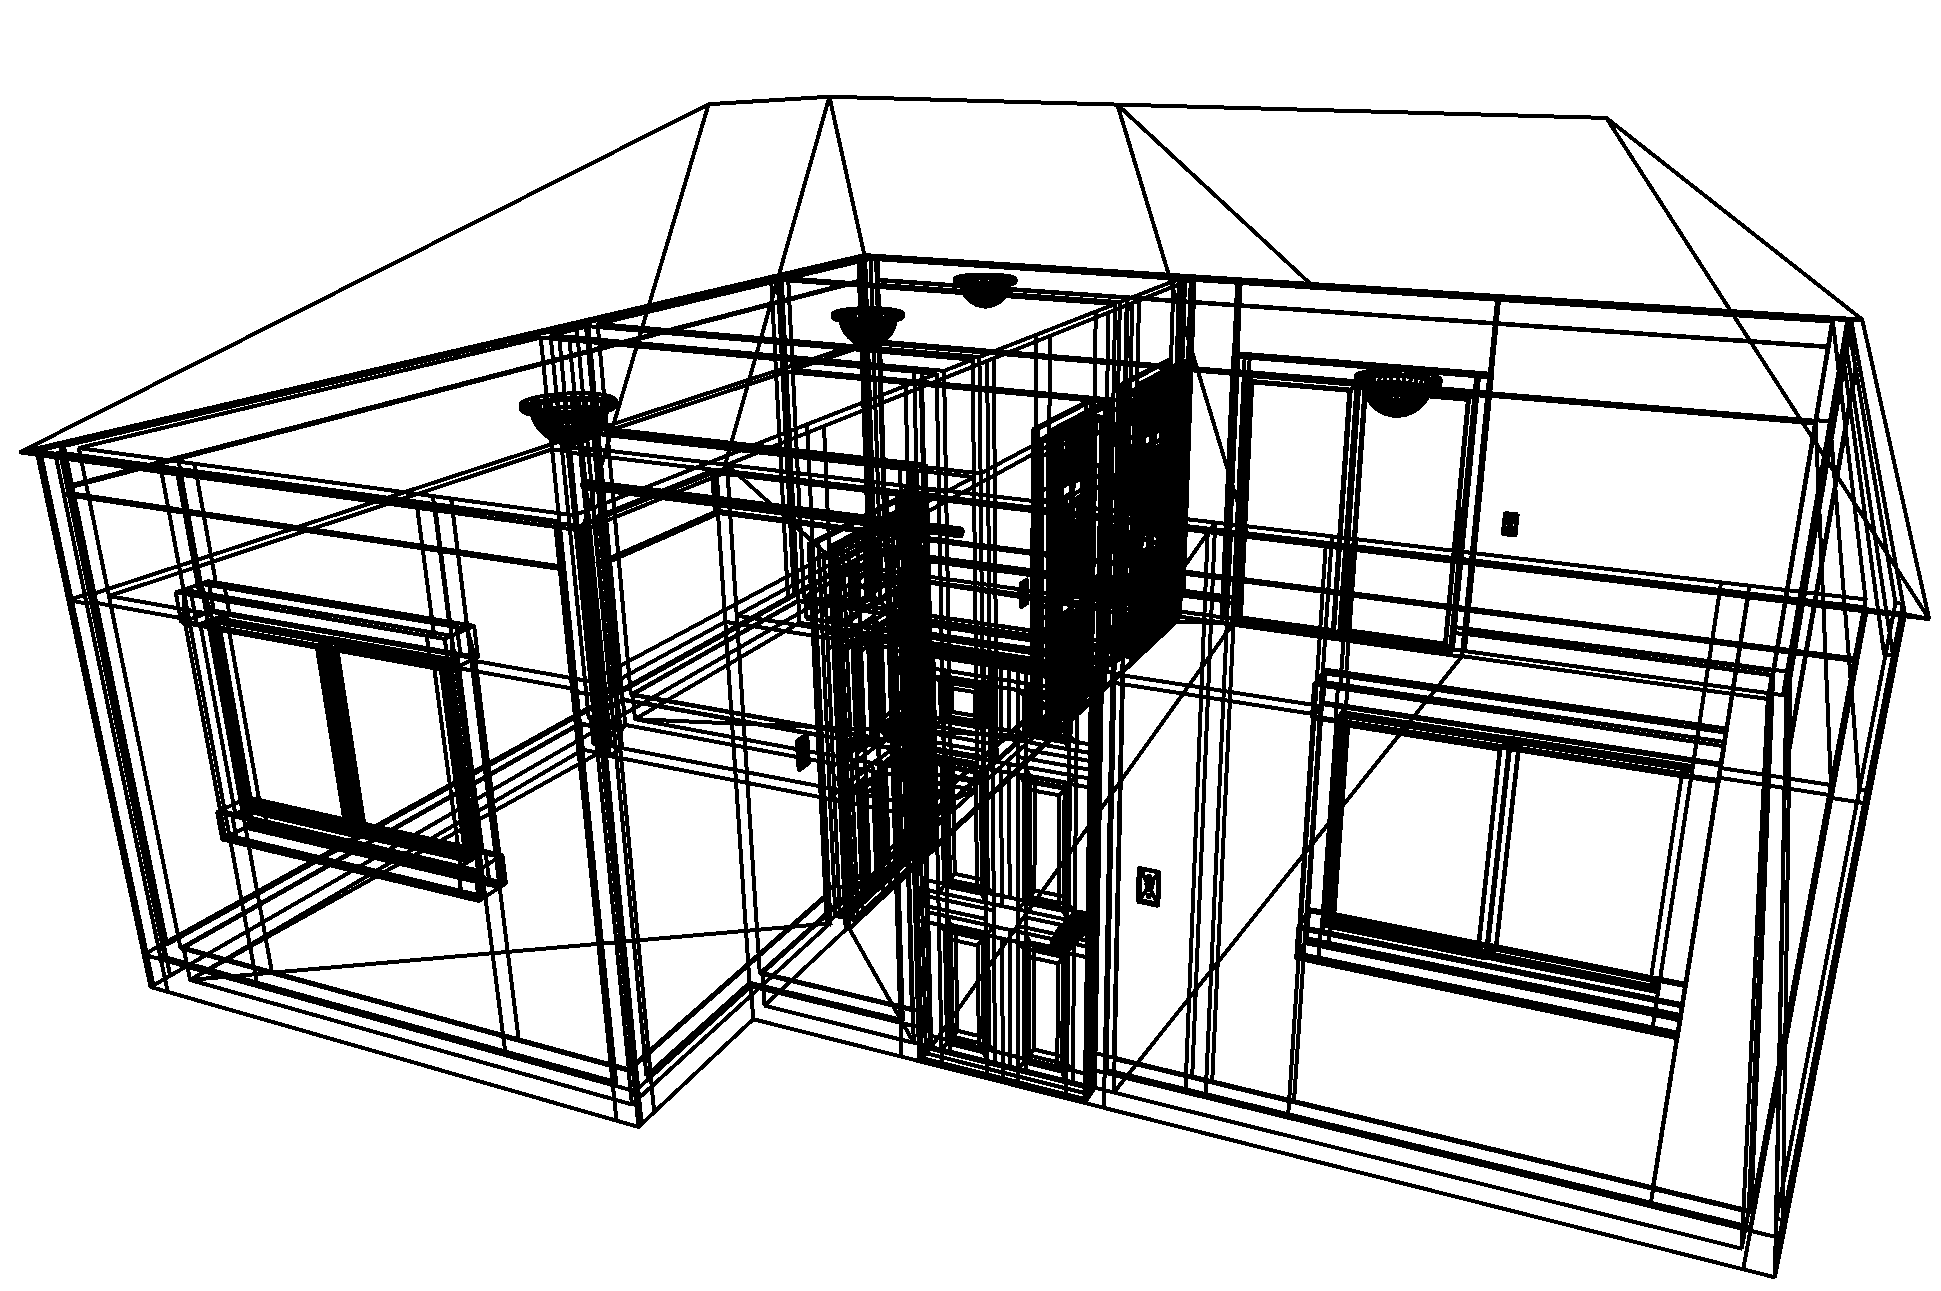
\includegraphics[width=\textwidth]{figures/experiments/house.png}
    \end{center}
    \caption[House with $K=8367$ obstacles]{House with $K=8367$ obstacles}
    \label{fig:house}
\end{figure}


\textbf{Sources $S_i$ and Receivers $R_j$}\newline
Receivers and sources can be specified in CSV files where each line represents the position of a source or a receiver. 
Format is \texttt{"x, y, z"}.
For now only positions are being loaded.

\section{Matryoshka Cube Test}
The purpose of the "Matryoshka Cube" test is to measure the simulation time of the Ray Tracer module with increasing number of objects $K$.
One property of the Matryoshka Cube is that most of paths checked obviously do not exist.
The current strategy ignores certain geometric conditions.
Future strategies can be evaluated with this test and therefore tell if an improvement is measurable or not.
Evaluating \eqref{eq:complex} for $L=3$ and for $K \gg M,N$ it is clear that the problem is of order $O(K^3)$ with the current strategy.

For the Matryoshka Cube Test a single receiver $R_1$ and a single source $S_1$ at position $(0,0,0)$ will be used.
The number of $K$ objects will be doubled in each step and the simulations will run with reflection orders $L=2$ and $L=3$.
In \tabref{tab:matryoshka} you can see the results of that test.

\begin{table}[H]
    \centering
    % spacing in table
    \ra{1.3}
    \begin{tabular}{llll}
      \toprule
      $X$ & $K$ & $L=2$ [s] & $L=3$ [s] \\ \midrule
      1	& 6 & 0.03	& 0.071	         \\
      2	    & 12	& 0.034	& 0.072 	 \\
      4	    & 24	& 0.034	& 0.078	   \\
      8	    & 48	& 0.03	& 0.12	   \\
      16    & 96	& 0.032	& 0.501	   \\
      32    & 192	& 0.042	& 3.268	   \\
      64    & 384	& 0.09	& 25.094	 \\
      128   & 768	& 0.253	& 193.004  \\
      \bottomrule
    \end{tabular}

    \caption[Matryoshka Cube Test Results]{Matryoshka Cube Test Results}
    \label{tab:matryoshka}
\end{table}


First thing to notice is that for second order reflections $L=2$ we still get reasonable run times for $K=768$.
Adding another layer of paths by increasing the allowed reflection order to $L=3$ the weight of the problem becomes clear.
For $K>32$ the factor of $2^3=8$ can be seen in the simulation time.

Nonetheless this was an expected behavior for the chosen strategy and for an increasing number of obstacles and it leaves room for improvement.

\section{Tube Test}
The purpose of the "Tube" test is to measure the simulation time of the Path Sampler module with increasing number of paths and sampling time.
One important property of the Tube is that for every pair $(S_i, R_j)$ which lies between the floor and the ceiling the maximum number of paths exist.
The maximum number of paths is given by \eqref{eq:complex}.
Using this equation and inserting $K=2, L=3$ for the Tube we can get following number of paths for $M$ sources and $N$ receivers:

\begin{equation}
    C_3 = M \cdot N \cdot (1 + 2 \cdot 3) = 7 \cdot M \cdot N
\end{equation}

In \tabref{tab:tube} you can see the results for a single receiver $R_1$ at position $(0,0,0)$ and $M$ sources distributed evenly across the room, between the floor and the ceiling.
It includes runs for different sampling durations $t$.

\begin{table}[H]
    \centering
    % spacing in table
    \ra{1.3}
    \begin{tabular}{lllll}
      \toprule
      $M$ & $C_3$ & $t=0.1 [s]$ & $t=0.3 [s]$ & $t=0.5 [s]$ \\ \midrule
      1 & 7 & 0.008 & 0.010 & 0.016  \\
      8 & 56 & 0.027 & 0.076 & 0.128   \\
      27 & 189 & 0.086 & 0.261 & 0.438   \\
      64 & 448 & 0.203 & 0.618 & 1.034   \\
      125 & 875 & 0.397 & 1.218 & 2.044   \\
      216 & 1512 & 0.695 & 2.132 & 3.571   \\
      343 & 2401 & 1.114 & 3.417 & 5.731   \\
      512 & 3584 & 1.687 & 5.138 & 8.555   \\
      729 & 5103 & 2.394 & 7.309 & 12.235   \\
      1000 & 7000 & 3.286 & 10.284 & 16.933  \\
      \bottomrule
    \end{tabular}

    \caption[Tube Test Results]{Tube Test Results}
    \label{tab:tube}
\end{table}


We can see a linear behavior for increasing number of sources $M$ and increasing sampling time $t$.
This was expected given the complexity relation between sources, receivers and number of objects in \eqref{eq:complex}.

For implementation details check the source code of \texttt{test/TestTube.cpp}.

\section{LOS Estimator}
The LOS (line-of-sight) multilateration estimator shows how ARTS can be used to estimate the location of $M$ sources using $N \geq 4$ receiver nodes in the Reference Room.
The implementation is based on Zhou Yu's paper \cite{zhou2009efficient}.
The main idea of multilateration is to use a predefined set of receivers $R$ and estimate the location to an unknown source $S_i$ by using the travel time from the source to each receiver node.
This of course requires that the source is in line-of-sight of each receiver node.
The minium number of receivers for such a system in 3D space is 4.
More nodes can be added to minimize the error of the estimated location.

In the current implementation $M=1000$ sources are evenly distributed in the Reference Room.
For the LOS localization system the receivers $R = \{ R_1(0,0,0)$, $R_2(1,0,0)$, $R_3(0,1,0)$, $R_4(0,0,1) \}$ will be used.
The simulator will run only for direct paths $L=0$ because reflections are not needed and therefore would be discarded anyway.
By getting the room impulse response (RIR) mentioned in \secref{sec:modelSimplification} the travel time can easily be obtained.

\textbf{Output of the test:}
\begin{verbatim}
# of Paths: 4000
0-Paths: 4000
# of Samples: 400000000
Error avg: 0.000452092
Error min: 0
Error max: 0.00141538
\end{verbatim}

For the evaluation of the estimated locations the euclidean distance has been used.
Since we didn't add any noise to our simulation the error is expected to be very low.
The seen error is due to sampling inaccuracies which is an effect that can not be avoided.
The magnitude of the error is in this particular case negligible.

For implementation details check the source code of \texttt{test/TestLOSEstimator.cpp}.

    \chapter{Conclusion and Future Work}\label{chap:conclusion}
The Acoustic Ray Tracing approach seems very promising for indoor localization and mapping applications.
With ARTS a very useful and scalable tool for indoor environments has been created.
The modular architecture provides flexibility and lots of room for exploration.
The tool can be used on any platform by containerizing it with tools like Docker\cite{docker}.
This should be considered especially for future releases including GPU acceleration.
The use of industry standard 3D model formats allows any user to rapidly design and test arbitrary environments with tools of their choice.
Once creating these 3D models can be automated or accelerated, the need for a tool like ARTS for indoor localization or mapping applications becomes indispensable.

There are certain functionalities, improvements and features missing which might be necessary and great to add:

The run-time of the Ray Tracing Module is still slow and it has a lot of potential to be optimized.
The same can be said for the Path Sampler.
Since these parts of the algorithm can be parallelized, we are almost guaranteed to see an improvement in performance by using a GPU.
This would most likely require moving away from CGAL\cite{cgal} as it currently doesn't support accessing CGAL objects from multiple threads.
The best solution would probably be to use data structures and API calls from libraries like OpenCL or Vulkan \cite{vulkan}, which support multiple GPUs, even on embedded platforms.
The docker functionality for such solutions is probably limited or currently not possible.
CUDA\cite{cuda} seems to work for Linux based systems but limited to NVIDIA GPUs.

Another area worth exploring is possibly leveraging the compute power of NVIDIA's new RTX GPUs\cite{nvidia}.
If they can do light ray tracing in real-time it will probably work for acoustics as well.

The proposed model does not include effects like scattering, diffraction and the influence of signal frequency.
Continued work that takes these effects into consideration would likely yield a more realistic model, especially in regards to noise generation.
Given the modular architecture, it should be possible to gradually add these effects to the model.

    \chapter{Acknowledgments}

First and foremost, I would like to thank my loving and amazing wife Livia.
She has been supportive in every possible way and for that I will always be grateful.\newline
I want to thank \firstexaminer{} for giving me the opportunity to work on such an interesting and challenging topic. His inputs and presentations were really inspiring and gave me the right direction to follow.\newline
Furthermore I would like to thank the members of the ILDARS team for giving me important inputs when I started my thesis.\newline
I also want to thank \secondexaminer{} for agreeing to take the position as second examiner on short notice.\newline
Last but not least I would like to thank my friends Vasili Massaras and Mike Fischer for proofreading this thesis and dealing with my silly English mistakes.

    
    % If you want a list of your ToDos at the end of the document
    % don't forget to remove before submission!
    %% place it somewhere in the document
\chapter*{ToDo Counters}
\newcounter{ct}%
To Dos: \arabic{todos}; \hspace{1em}%
\setcounter{ct}{0}%
\whiledo {\value{ct} < \value{todos}}%
{%
	\stepcounter {ct}%
    \ref{todo \thect}%
	\ifnum\value{ct} = \value{todos}{}\else{, }\fi
}

Parts to extend: \arabic{extends}; \hspace{1em}%
\setcounter{ct}{0}%
\whiledo {\value{ct} < \value{extends}}%
{%
	\stepcounter {ct}%
	\ref{extend \thect}%
	\ifnum\value{ct} = \value{extends}{}\else{, }\fi
}

Draft parts: \arabic{drafts}; \hspace{1em}%
\setcounter{ct}{0}%
\whiledo {\value{ct} < \value{drafts}}%
{%
	\stepcounter {ct}%
	\ref{draft \thect}%
	\ifnum\value{ct} = \value{drafts}{}\else{, }\fi
}


    \bibliographystyle{ieeetr}
    \bibliography{bib/general, bib/localization, bib/mapping, bib/ray_tracing, bib/web}
    % bibliography is not in the table of contents per default, add it manually
    % enable the \renewcommand for german header
    % \renewcommand{\bibname}{Literaturverzeichnis}
    \addcontentsline{toc}{chapter}{Bibliography}
    \newpage
    \thispagestyle{empty}
    \mbox{}


\end{document}
